%-*- coding=utf-8 -*-
\documentclass[UTF8]{ctexart}
\usepackage{geometry}
\CTEXsetup[format={\Huge\bfseries}]{section}
\CTEXsetup[format={\LARGE\bfseries}]{subsection}
%\usepackage{titlesec}
\geometry{left=3.18cm,right=3.18cm,top=2.54cm,bottom=2.54cm}
\usepackage{graphicx}
\pagestyle{plain}	
% \usepackage{booktabs}
% \usepackage{subfigure}
\usepackage{setspace}
\usepackage{float}
\begin{document}
	\begin{center}
		\quad \\
		\quad \\
		\heiti \fontsize{45}{17} 高级网络编程
		\vskip 2.0cm
		\heiti \fontsize{39}{17} 实验报告	
	\end{center}
	\vskip 3.5cm
	\begin{quotation}
		\par\setlength\parindent{8.5em}
		\quad 
		\heiti 
		
		实验名称:腾讯会议传输方式分析
		
		实验日期:2020年5月29日
	
		学生姓名:黄文政
		
		学\hspace{0.72cm}号:71Y17111
		
		\vskip 2cm
		\centering
	\end{quotation}
	
\newpage
\songti \fontsize{13}{13}
\large
\section*{一、实验目的}

1. 通过抓包方式分析腾讯会议的传输方式


\section*{二、实验环境}
windows 10、wireshark

\section*{三、实验内容}
\subsection*{\textbf{通过抓包方式分析腾讯会议的传输方式
}}
\subsection*{主要过程}

1. 在会议中启动wireshark,筛选UDP包

2. 观察出主机持续接收大量来自同一地址的UDP包,初步判断这些包即为腾讯会议的流量包

\begin{figure}[H]
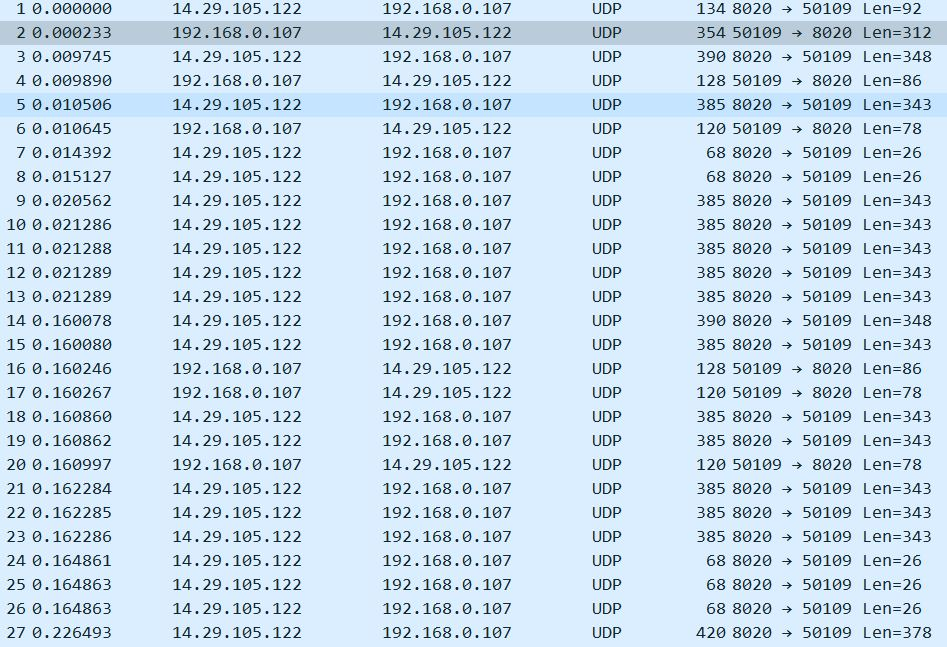
\includegraphics[width=\textwidth]{pic/tx1.jpg}
\caption{UDP包}
\end{figure}

3. 分析包的内容,查看到发送和接收都为单播

\begin{figure}[H]
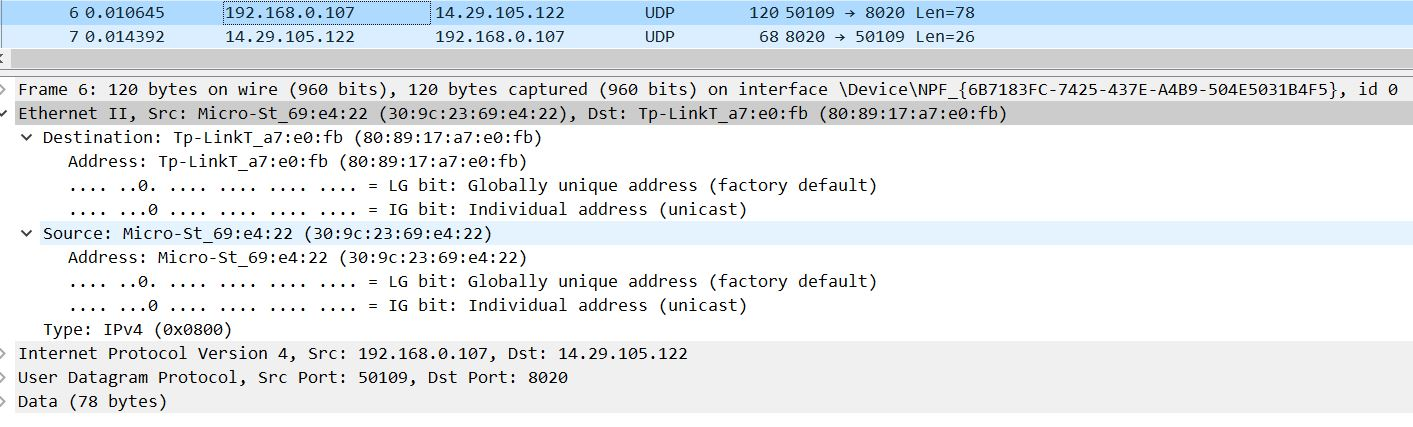
\includegraphics[width=\textwidth]{pic/txsend.jpg}
\caption{发送}
\end{figure}

\begin{figure}[H]
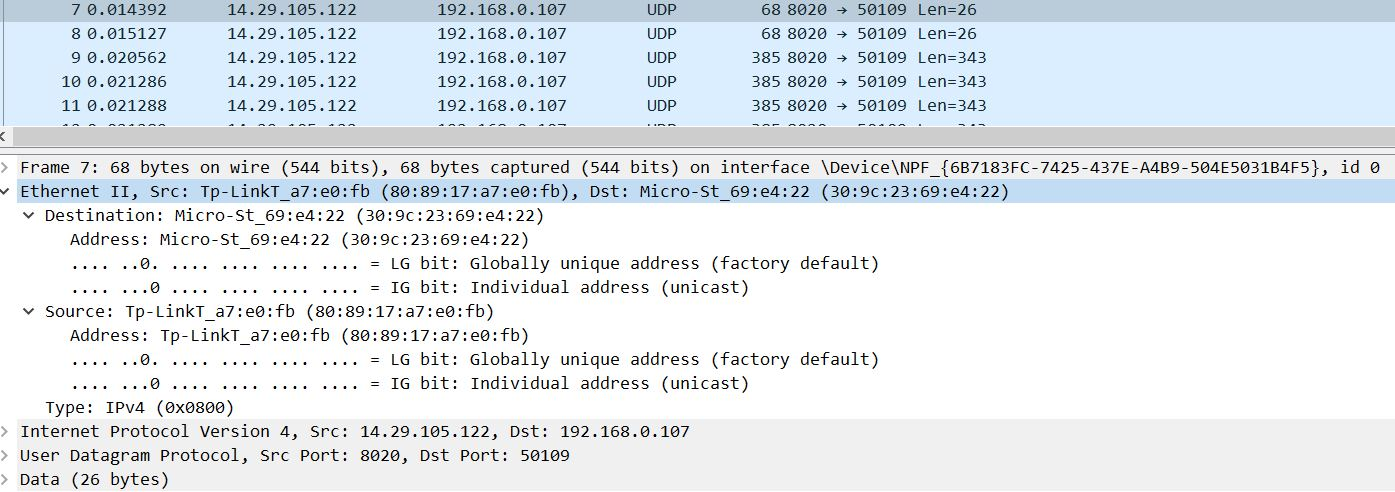
\includegraphics[width=\textwidth]{pic/txrecv.jpg}
\caption{接收}
\end{figure}



\section*{四、实验总结}

腾讯会议使用了UDP单播的方式发送数据包。

\end{document}